\documentclass[10pt]{article}
\usepackage[utf8]{inputenc}
\usepackage[includehead, headheight=10mm, margin=15mm ]{geometry}
\usepackage{amsmath}
\usepackage{amsthm}
\usepackage{amsfonts}
\usepackage{xcolor}
\usepackage{graphicx}
\usepackage{titling}
\usepackage{fancyhdr}

\title{APPM 4600 Homework 1}
\author{Edward Wawrzynek}
\date{6 September 2024}

\newcommand*{\dif}{\mathop{}\!\mathrm{d}}

\makeatletter
\def\@maketitle{%
  \newpage
  \null
  \vskip 1em%
  \begin{center}%
  \let \footnote \thanks
    {\LARGE \@title \par}%
    \vskip 1em%
    {\normalfont \@date}
  \end{center}%
  \par
  \vskip 1em}
\makeatother

\begin{document}

\pagestyle{fancy}
    \fancyhf{} % clear all header and footer fields
    \fancyhead[L]{\thetitle}
    \fancyhead[R]{\theauthor}

\makeatletter
\begin{center}
    {\Large \@title}
    \vskip 1mm
    {\normalfont \@date}
    \vskip 1em
\end{center}
\makeatother

\begin{enumerate}
    \item \begin{enumerate}
        \item A plot of \(p(x) = x^9 - 18x^8 + 144x^7 - 672x^6 + 2016x^5 - 4032x^4 + 5376x^3 - 4608x^2 + 2304x - 512\) evaluated via its expanded form is shown below.
        \begin{center}
            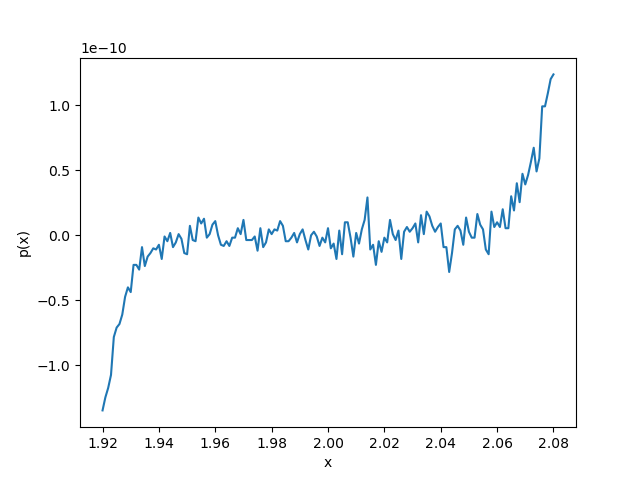
\includegraphics[width=0.5\textwidth]{hw1_1_eval1.png}
        \end{center}
        \item A plot of \(p(x) = (x-2)^9\) evaluated in that form is shown below.
        \begin{center}
            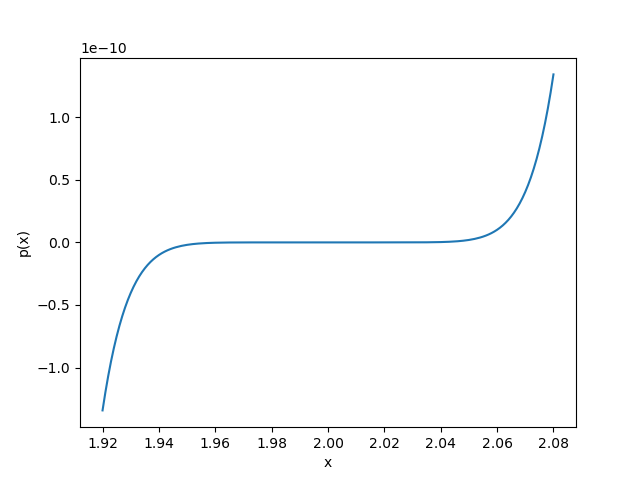
\includegraphics[width=0.5\textwidth]{hw1_1_eval2.png}
        \end{center}
        \item The second plot is much closer to being correct. When evaluated via the expanded form, the high order terms (which largely cancel near \(x \approx 2\)) become very large and cause a loss of precision in the floating point representation of the value of the function.
    \end{enumerate}
    \item \begin{enumerate}
        \item We can evaluate as \begin{align*}
            \sqrt{x+1}-1 &= \frac{(\sqrt{x+1}-1)(\sqrt{x+1}+1)}{\sqrt{x+1}+1} \\
            &= \frac{x+1 -1}{\sqrt{x+1}+1} \\
            &= \frac{x}{\sqrt{x+1}+1}.
        \end{align*}
        \item We can evaluate via the sum to product identity as \begin{align*}
            \sin(x) - \sin(y) &= 2\sin \left(\frac{x-y}{2}\right)\cos  \left( \frac{x+y}{2} \right).
        \end{align*}
        \item We can evaluate as \begin{align*}
            \frac{\cos \left( x \right)-1}{\sin  \left( x \right)} &= \frac{(\cos \left( x \right)-1)(\cos  \left( x \right) + 1)}{\sin  \left( x \right)(\cos  (x) + 1)} \\
            &= \frac{\cos ^2(x) - 1}{\sin  \left( x \right)(\cos  (x) + 1)} \\
            &= \frac{\sin  (x)}{cos(x) + 1}.
        \end{align*}
    \end{enumerate}
    \item \begin{enumerate}
        \item We have the Taylor expansion \begin{align*}
            P_2(x) &= (1 + x + x^3)\cos(x) \\
            &= (1 + x + x^3)\left( 1 - \frac{x^2}{2!} + \frac{x^4}{4!} + \dots \right) \\
            &\approx 1 + x - \frac{1}{2}x^2.
        \end{align*}

        We evaluate at \(x=0.5\) and find \(P_2(0.5) = 1.375\). From Taylor's inequality, we have that the error is bound as \begin{align*}
            |f(0.5) - P_2(0.25)| \leq \frac{|M|}{3!}(0.5)^3,
        \end{align*} where \(|f^{(3)}(x)| \leq M\) on \(x \in [0, 0.5]\). We have \begin{align*}
            f'(x) &= (1+3x^2)\cos(x) - (1+x+x^3)\sin  (x) \\
            f''(x) &= 6x\cos(x) - 2(1+3x^2)sin(x) + (1+x+x^3)\cos  (x) \\
            f'''(x) &= 6\cos(x) -6x\sin(x) - 12x\sin(x) -(1+3x^2)\cos(x) - (1+x+x^3)\sin  (x),
        \end{align*}
        which we can bound as \(|f'''(x)| < 3\) on \(x\in[0, 0.5]\). Thus, our error bound is \begin{align*}
            |f(0.5) - P_2(0.25)| \leq \frac{3}{3!}(0.5)^3 = \left(\frac{1}{2}\right)^4 = 0.0625.
        \end{align*}

        The actual error is \begin{align*}
            |f(0.5) - P_2(0.5)| = |1.426071 - 1.375| = 0.05107,
        \end{align*} which is less than our error bound.

        \item From Taylor's theorem, we have the error bound \begin{align*}
            |f(x) - P_2(x)| \leq \frac{|M|}{3!}(x)^3,
        \end{align*} where \(|f^{(3)}(x)| \leq M\) on \(x \in [0, x]\). If we have \(|x| < 0.5\), we can use \(M=3\) from before.

        \item We have \begin{align*}
            \int_0^1 f(x)\dif x &\approx \int_0^1P_2(x)\dif x \\
            &= \int_0^1 \left( 1+x-\frac{1}{2}x^2 \right)\dif x \\
            &= \left( x+\frac{1}{2}x^2-\frac{1}{6}x^3 \right)_0^1 \\
            &= \frac{4}{3}.
        \end{align*}

        \item We known that \(|f^{(3)}(x)| \leq 16\) on \(x \in [0, 1]\), so the error is bounded by \begin{align*}
            E &\leq \int_0^1 \frac{16}{3!}x^3 \dif x \\
             &= \frac{8}{3} \left( \frac{1}{4}x^4 \right)_0^1 \\
             &= \frac{2}{3}.
        \end{align*}
    \end{enumerate}
    
    \item 
    \begin{enumerate}
    \item The "bad" root will be the one where the numerator of the quadratic formula is near zero. Since \(b\) is negative, this is the root \begin{align*}
        r_2 = \frac{-b - \sqrt{b^2-4ac}}{2a}.
    \end{align*}

    We compute the square root to three decimal places, \begin{align*}
        \sqrt{b^2-4ac} = \sqrt{56^2-4} \approx 55.964,
    \end{align*} and find root \begin{align*}
        r_2 = \frac{1}{4}\left( 56 - 55.964 \right) = 0.018.
    \end{align*} The actual root is \(r_2 \approx 0.01786284073\), which is 0.77\% error.

    The other root is computed as \begin{align*}
        r_1 = \frac{-b + \sqrt{b^2-4ac}}{2a} = \frac{56 + \sqrt{56^2 - 4}}{2} \approx \frac{56 + 55.964}{2} \approx 55.982,
    \end{align*} which is a 0.00025\% error from the real root.

    \item We have that \begin{align*}
        ax^2 + bx + c &= (x-r_1)(x-r_2) \\
        &= x^2 - (r_1+r_2)x+r_1r_2,
    \end{align*} which implies that \(b=-r_1-r_2\) and \(c=r_1r_2\). These give the two relations \begin{align*}
        r_2 &= -b - r_1 \\
        r_2 &= \frac{c}{r_1}.
    \end{align*}

    The second gives a better estimate for the root, \begin{align*}
        r_2 &= \frac{c}{r_1} \approx \frac{1}{55.982} = 0.01786288450,
    \end{align*} which is a 0.00025\% error from the real root.
    \end{enumerate}

    \item \begin{enumerate}
        \item The absolute error is bounded as \begin{align*}
            |\Delta y| \leq |\Delta x_1| + |\Delta x_2|,
        \end{align*} and the relative error as \begin{align*}
            \frac{|\Delta y|}{|y|} \leq \frac{|\Delta x_1| + |\Delta x_2|}{|x_1-x_2|}.
        \end{align*} The relative error is large when \(x_1\) and \(x_2\) are close in value, and the \(\Delta x\) terms become comparable in magnitude to \(x_1-x_2\).
        \item We can evaluate as \begin{align}\label{eq:eval_1}
            \cos(x+\delta ) - \cos  (x) &= -2\sin \left( \frac{2x+\delta }{2} \right)\sin  \left( \frac{\delta}{2} \right).
        \end{align}

        A plot of the difference in the evaluation of the two expressions is shown below for \(x=\pi\) and \(x=10^6\).

        \begin{center}
            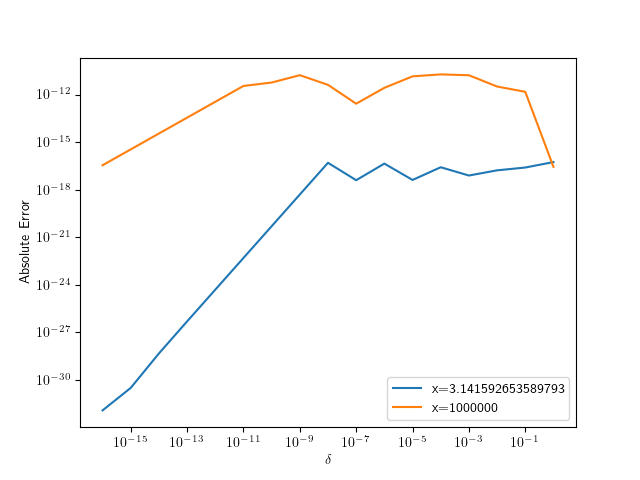
\includegraphics[width=0.5\textwidth]{hw1_5_pi.png}
        \end{center}

        Notice that for \(x=\pi\) and \(\delta \) small, the difference is linear with \(\delta \)---the non-corrected expression evaluates to zero, and the difference is simply the value of the corrected expression. As \(\delta\) increases the subtraction becomes less problematic and the absolute error between the two expressions stops growing. For \(x=10^6\), the two terms that are subtracted are large and the error is significant even for small \(\delta \).

        \item Let \(f(x) = \cos  (x)\). We have the derivatives \begin{align*}
            f'(x) &= -\sin  (x) \\
            f''(x) &= -\cos  (x),
        \end{align*} so the Taylor expansion yields \begin{align*}
            \cos(x+\delta)-\cos(x) \approx -\delta\sin(x)-\frac{\delta^2}{2}\cos(x).
        \end{align*}

        We modify the second order term to be evaluated at \(x+\frac{\delta}{2}\), which splits the range \([x, x+\delta ]\) over which we concerned about evaluation, yielding \begin{align}\label{eq:eval_2}
            \cos(x+\delta)-\cos(x) \approx -\delta\sin(x)-\frac{\delta^2}{2}\cos(x+\frac{\delta}{2})
        \end{align}

        The absolute difference between evaluating via \eqref{eq:eval_1} and \eqref{eq:eval_2} is plotted below.

        \begin{center}
            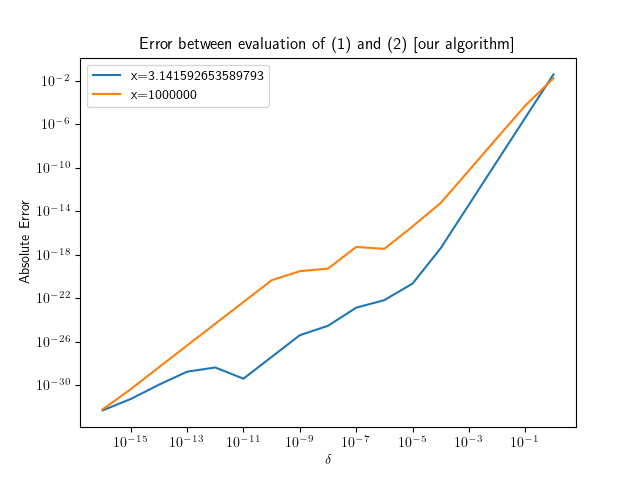
\includegraphics[width=0.5\textwidth]{hw1_5_our_algorithm.png}
        \end{center}

        Notice that our algorithm \eqref{eq:eval_2} has low absolute different for small \(\delta \) for both \(x=\pi\) and \(x=10^6\). It performs poorly with large \(\delta\), where the higher order terms we dropped from the Taylor expansion become more significant.
            
    \end{enumerate}

\end{enumerate}


\end{document}